\input{header}

\AtBeginSubsection[]
{
	\begin{frame}<beamer>
		\frametitle{Outline}
		\tableofcontents[current,currentsubsection]
	\end{frame}
}

\begin{document}

\begin{frame}[allowframebreaks] \frametitle{Chapter 4: Decidability}
  \begin{itemize}
\item Now we have algorithms
\item We want to check problems solvable or not by computers

\item Need a TM to decide it

\item [] i.e., accept/reject in a finite number of steps

\item We will show some examples
  
\end{itemize}\end{frame}

\begin{frame}[allowframebreaks] \frametitle{Acceptance Problems for DFA}
\begin{equation*}
  A_{DFA}=
\{\langle  B,w\rangle\mid B \mbox{ is a DFA that accepts } w\}
\end{equation*}
  \begin{itemize}
\item $\langle  B,w\rangle$ is the input
\item [] Note that a DFA can be represented as a string $(Q, \Sigma, \ldots)$
\item Is $A_{DFA}$ decidable?

\item Idea: input $\langle  B,w\rangle$
  \begin{enumerate}
  \item simulate $B$ on $w$
  \item ends in an accept state $\Rightarrow$ accept

otherwise $\Rightarrow$ reject

  \end{enumerate}
\end{itemize}\end{frame} \begin{frame}[allowframebreaks] \frametitle{Proof of $A_{DFA}$}
  \begin{itemize}
  \item Put
    \begin{equation*}
    B=\langle  Q,\Sigma,\delta,q_0,F\rangle
  \end{equation*}
into a tape
\item Check if $w\in \Sigma^*$ and $B$ a valid DFA
\item Simulate $w$ according to $\delta$
\item After processing the last element of $w$, check if in a final state

\end{itemize}\end{frame} \begin{frame}[allowframebreaks] \frametitle{$A_{NFA}$}
\begin{equation*}
  A_{NFA}
=\{\langle  B,w\rangle \mid B \mbox{ is an NFA that accepts } w\}
\end{equation*}
  \begin{itemize}
\item We can convert $B$ to a DFA and 
use the procedure for $A_{DFA}$
\item It's like to use the procedure for $A_{DFA}$
as a subroutine

\end{itemize}\end{frame} \begin{frame}[allowframebreaks] \frametitle{$A_{REX}$}
\begin{equation*}
  A_{REX}
=\{\langle  R,w\rangle \mid R: \mbox{ regular expression generates } w\}
\end{equation*}
  \begin{itemize}
\item It's similar
\item We convert $R$ to a DFA first
\item Recall that we had a procedure to convert $R$ to an NFA. Then we
  can convert the NFA to a DFA
\item The key is that the conversion is a \alert{finite} procedure
\end{itemize}\end{frame} \begin{frame}[allowframebreaks] \frametitle{$E_{DFA}$}
\begin{equation*}
  E_{DFA}
=\{\langle  A\rangle 
\mid A: DFA, L(A)=\emptyset\}
\end{equation*}
  \begin{itemize}
\item i.e. $A$ accepts nothing
\item Idea:

\item [] DFA accepts something

$\Leftrightarrow$ reaching a final state from $q_0$ 
after several links
\item procedure
  \begin{enumerate}
  \item mark $q_0$
  \item repeat until no new state marked

\qquad mark all 
\begin{equation*}
  a\rightarrow b,
\end{equation*}
\qquad where $a$ has been marked
\item if no $q\in F$ marked, accept.
otherwise, reject
  \end{enumerate}
\item Example: a state diagram with 3 nodes and the following connections
  \begin{equation*}
    1\rightarrow 2, 3
  \end{equation*}
  Marked states in running the procedure
  \begin{equation*}
    \begin{split}
& 1  \\
& 1 2\\
& 1 2\\
\end{split}
\end{equation*}
\item Each iteration: at least one new state marked
\item At most $n$ iterations: $n$: \# states
\end{itemize}\end{frame} \begin{frame}[allowframebreaks] \frametitle{$EQ_{DFA}$}
\begin{equation*}
  EQ_{DFA}
=\{\langle  A,B\rangle \mid A, B: DFAs, 
L(A)=L(B)\}
\end{equation*}
  \begin{itemize}
\item $EQ_{DFA}$ is decidable
\item Idea for the proof:

\item Let a DFA C be the exclusive or of A and B

\item [] If
  \begin{equation*}
  L(A)=L(B)
\end{equation*}
then
\begin{equation*}
  L(C)=\emptyset
\end{equation*}

\begin{center}
  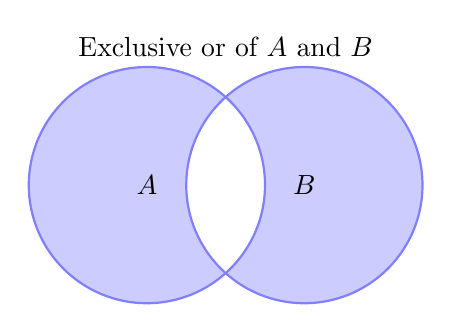
\begin{tikzpicture}
    [filled/.style={fill=blue!20, draw=blue!50, thick}, outline/.style={draw=blue!50, thick}]
    \draw[filled, even odd rule] (0,0) circle (1.5cm) node {$A$}
                                 (0:2cm) circle (1.5cm) node{$B$};
    \node[anchor=south] at (current bounding box.north) {Exclusive or of $A$ and $B$};
\end{tikzpicture}
\end{center}
{\small (latex source from
\url{https://texample.net/tikz/examples/set-operations-illustrated-with-venn-diagrams/})}

\item Formally
  \begin{equation*}
    L(C)
=(L(A)\cap \overline{L(B)})\cup
(\overline{L(A)}\cap L(B))
  \end{equation*}
\item 
$B$ DFA $\Rightarrow$ so is $\overline{B}$

\item $A, B$ DFA $\Rightarrow$ so is 
$A\cup B, A\cap B$

\item We then use $E_{DFA}$ to check if 
$  L(C)=\emptyset $ or not
\end{itemize}\end{frame}

\end{document}

%%% Local Variables:
%%% mode: latex
%%% TeX-master: t
%%% End:
